\section{Overview of the Recommenders Repository}

The repository is open-sourced under the MIT License. All the algorithms and utilities have been written in the Python programming language and the demonstrations are 
in the form of Jupyter notebooks.
The platforms supported are Linux and Windows. Some of the algorithms can take advantage of GPU resources if available 
and some others require a Spark environment \cite{meng2016mllib}. In Figure \ref{figure_structure} a diagram of the repository structure is shown.

\begin{figure}
  \centering
  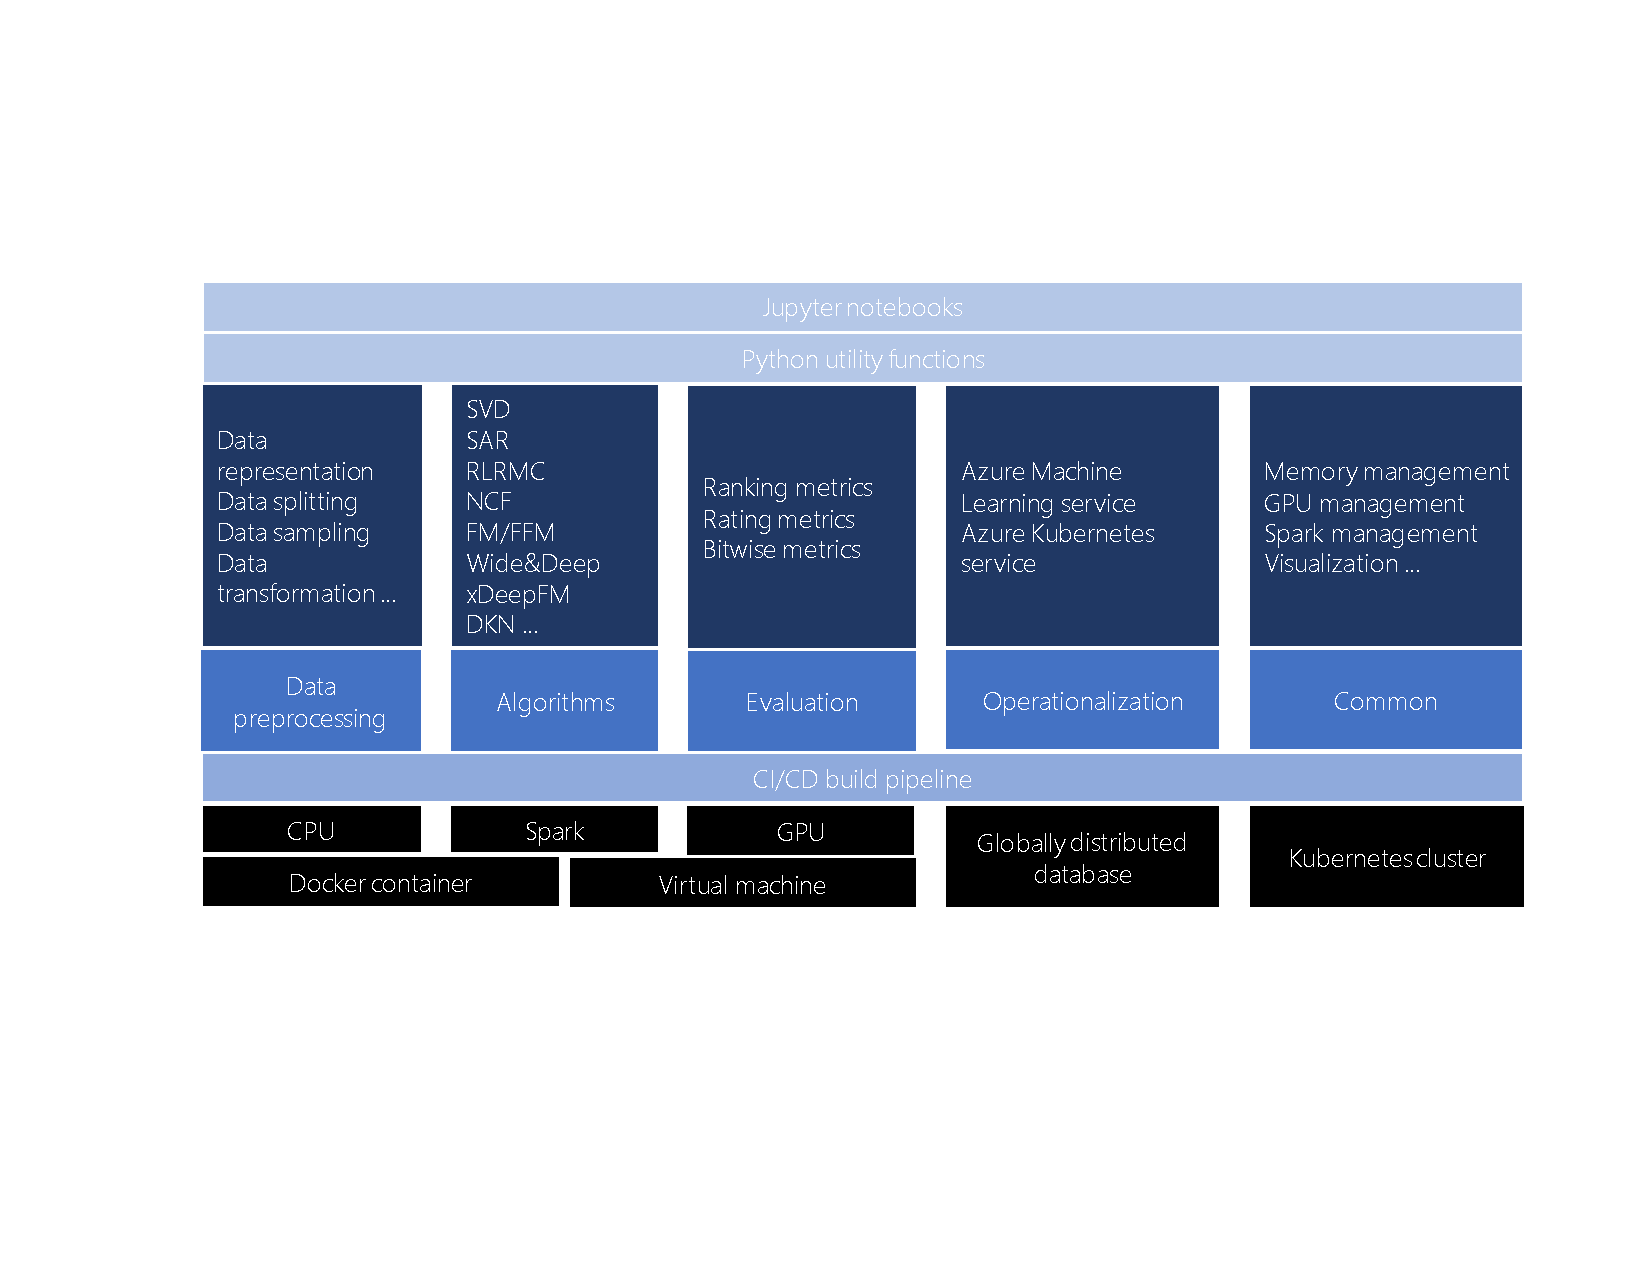
\includegraphics[width=\textwidth,keepaspectratio]{platform_diagram_crop.pdf}
  \caption{Microsoft Recommenders structure diagram. Layers from the bottom to the top are the underlying 
  infrastructure, build pipeline, recommendation tasks, utility functions, and example Jupyter notebooks.}
  \label{figure_structure}
\end{figure}

%Microsoft Recommenders is based on best practices for building recommendation systems, which have been learned from the 
%application of production-ready systems on Microsoft customers. As a consequence, we have followed an {\em end-to-end} approach, which 
%is not limited to just the training of an algorithm, but encompasses a number of components typical in a 
%recommendation pipeline like data preparation, model selection, evaluation and operationalization.
%
%Several utilities are provided in the 
%reco utils folder\footnote{\url{https://github.com/microsoft/recommenders/blob/master/reco_utils}} 
%to support common tasks such as loading datasets in the format expected by 
%different algorithms, evaluating model outputs, and splitting training/test data. 
%Implementations of several state-of-the-art algorithms are provided for self-study and 
%customization in one's own applications.
%
